\documentclass[journal]{IEEEtran}
\usepackage[T1]{fontenc}
\usepackage[utf8]{inputenc}
\usepackage{amsmath,amssymb}
\usepackage{graphicx}
\usepackage{booktabs}
\usepackage{array}
\usepackage{cite}
\usepackage{url}
\usepackage[hidelinks]{hyperref}
\hyphenation{Kuwa-hara}
\begin{document}
\title{Locality Matters: Tile-Consistent Content-Adaptive Anisotropic Kuwahara Filtering for Large-Canvas Abstraction}
\author{YingJie Wang%
\thanks{Y. Wang is with Handan College, Handan, Hebei, China.
E-mail: 717646407@qq.com. ORCID: 0009-0005-5898-0448.}%
}
\maketitle
\begin{abstract}
A filter whose parameter is computed from the whole image produces a different image when it is evaluated in tiles. We prove the condition behind this: if any quantity that can change a pixel's output is a non-degenerate whole-image functional, no finite overlap halo, and no single-pass streaming or out-of-core pass, reproduces the whole-image result. That separates the failure from support truncation, which a halo does fix, and yields a metric (TCE) that established quality measures do not respond to. The practical cost is metrological. Changing the evaluation harness moves a global-quantile variant by up to \(0.031\) SR and \(0.019\) SSIM, comparable to the largest quality gain we report, while the bounded-support operator LRS-AKF is unchanged at four decimals; four-method rankings invert in 15 of 40 cases. LRS-AKF is exactly tile-consistent on 141 of 144 benchmark images. The predicate also audits code we did not write: of seven published OpenCV 5.0.0 algorithms with bounds registered in advance, three are bit-exact inside their bound and two exceed it. An audit of four distributed anisotropic Kuwahara implementations found no whole-image reduction on their main support-selection path, so we state the result as a correctness criterion and a measurement protocol, not as a census of deployed practice.
\end{abstract}
\begin{IEEEkeywords}
image abstraction, anisotropic Kuwahara filter, tile consistency, out-of-core processing, reproducibility, evaluation protocol
\end{IEEEkeywords}
\section{Introduction}\label{sec:intro}

The anisotropic Kuwahara filter and its descendants produce painterly abstraction by comparing the variances of oriented sectors around each pixel and selecting the most homogeneous one~\cite{kuwahara1976,kyprianidis2009akf,kyprianidis2011msakf}. A fixed support is wrong in flat and in detailed regions, so a substantial literature adapts it: adaptive window selection~\cite{bartyzel2015adaptive,arya2024adaptive}, multi-scale variants~\cite{kyprianidis2011msakf}, depth-driven scale~\cite{ahn2010depth} and coherence-guided adaptivity~\cite{zang2015guided}. Each decides from a \emph{local} statistic. That statistic can nevertheless be normalised against an image-wide percentile before it is thresholded, which turns a local decision into a whole-image one.

This paper is about the correctness of that substitution. We do not claim it is common practice. Section~\ref{sec:audit} audits four distributed anisotropic-Kuwahara implementations at the expression that forms the parameter and finds no whole-image reduction on the main support-selection path of any of them. The pattern does occur in the two reference implementations we built, in the per-tile feature statistics of learned pipelines~\cite{buglakova2025tiling}, and in one published structure-repair branch whose mask threshold is an image-wide percentile. We therefore present it as a \emph{failure mode with a proof and a test}, not as a census of deployed code. What has not been stated is when such a substitution is exact, and what it costs when it is not.

\textbf{The property.} If a filter's parameter is a functional of the whole image, the output for a region depends on pixels outside that region. Tiled evaluation, mandatory whenever the image does not fit in memory~\cite{dash2022gigapixel,powell2010gigapixel} and standard in streaming and parallel pipelines, therefore produces a different image, not merely a lower-quality one. The benign half of this problem is well known. Overlap-tile evaluation obtains seamless results for arbitrarily large inputs~\cite{ronneberger2015unet}, and residual tiling effects are attributed to translation variance of strided or pooled operators and mitigated with larger tiles~\cite{reina2020tiling,huang2018tiling}. That is \textbf{support truncation}: a pixel near a tile edge lacks context, and a halo at least as wide as the operator's support repairs it exactly. The other half, \textbf{statistic non-locality}, survives every finite halo because the quantity that sets the parameter is computed from the entire image and changes from tile to tile.

\textbf{Why this matters beyond one operator.} Six established quality metrics are blind to a mismatch that moves 6.5--20.5\,\% of pixels by more than one 8-bit level. Because the mismatch is invisible to the metrics in current use, evaluation protocols that differ only in how the image is fed to the filter rank methods differently. On the same images, evaluating four filters tile-wise instead of whole-image inverts the ranking in 15 of 40 image-metric cases. A method can win a published comparison and lose in the pipeline that ships. The headline observation of this paper is that a global-quantile variant's quality figures move by up to \(0.019\) SSIM when the harness changes, about the size of the largest quality gain we report, while a bounded-support operator's published numbers do not move at the precision at which they are reported.

\textbf{Contributions.} (1) A taxonomy with a proof: a sufficient condition for exact tile consistency (Proposition~1, Section~\ref{sec:theory}) and a violation condition for whole-image functionals (Proposition~2), together with a measured correction to the sharp reading of Proposition~1. (2) An instrument: tile-consistency error, its border-band decomposition, grid-line visibility and a rank-inversion test, validated at three scales. (3) An operator, LRS-AKF, that satisfies the condition and is exactly tile-consistent on 141 of 144 benchmark images. (4) A metrological result: the portability of published numbers under a change of evaluation harness, measured on four operators and seven third-party algorithms. (5) A source-level audit of four distributed implementations, reported as a negative result that bounds the paper's own prevalence claim.

\section{Related work}\label{sec:related}

Tiling is the standard answer to an image that does not fit in memory~\cite{dash2022gigapixel,powell2010gigapixel}. The overlap-tile strategy was introduced to obtain seamless predictions~\cite{ronneberger2015unet}; residual effects were attributed to pooling and strided convolutions~\cite{reina2020tiling,huang2018tiling}; tile size and overlap are otherwise treated as configuration to be chosen~\cite{cira2024tile,mihajlovic2025sahi,akyon2022sahi}. These are class-A diagnoses in our terms: context missing at a border, repaired by more context. Closest to our mechanism, Buglakova et al.~\cite{buglakova2025tiling} trace tiling artefacts in sliding-window inference to feature-normalisation layers whose statistics are computed per tile and fix them by a normalisation whose test-time statistics are not tile-dependent. The response is an empirical swap of one layer for another, with no statement of \emph{when} a tiled evaluation equals the untiled one.

Three adjacent fields supply precedents that a reviewer would otherwise raise. Adaptive histogram equalisation computes its transfer function from block-wise histograms and interpolates between block centres~\cite{pizer1987clahe}, which is our design rule applied to contrast enhancement; it does not state when a partition reproduces the untiled result, and its block grid becomes part of the operator. Wavelet coding removes tile-boundary artefacts by point-symmetric extension and odd tile sizes~\cite{kharitonenko2002wavelet,wei2005tile}, the canonical class-A repair. Exact tile-based inference derives a required halo from a network's receptive field~\cite{majurski2021exact}, the same condition as Proposition~1 for a different operator class. One further precedent keeps a global coupling and still fits in memory: streaming multigrid solves a gradient-domain system in two out-of-core passes~\cite{kazhdan2008smg}. That is a solver-level fix, not a parameter-level one, and it does not claim that independent tiles reproduce the global solution. Bounded memory and bounded support are different properties; only the second survives an arbitrary partition.

Percentile normalisation also appears in contrast normalisation, auto-levels, histogram matching and, in learned pipelines, instance statistics computed on a thumbnail of the whole image~\cite{chen2022urst}. Streaming quantile summaries~\cite{greenwald2001gk} make a global statistic cheap but not local, since a tile's value still depends on other tiles. None of this literature provides a criterion under which a partition reproduces the whole-image evaluation, or an error measure that would let a reader check.

\section{Tile consistency}\label{sec:theory}

Let \(I\in\mathbb R^{H\times W\times 3}\) be an image, \(f\) an operator, \(\mathcal P_n\) the uniform \(n\times n\) partition into tiles, and \(f_{\mathcal P,h}\) the tile-wise evaluation with overlap halo \(h\): each tile \(T\) is extended by \(h\) pixels, \(f\) is applied, and only the pixels of \(T\) are kept.

\textbf{Definition 1 (tile consistency).} \(f\) is tile-consistent if for every image \(I\) there is \(h^*(I)\) such that for all \(n\) and all \(h\ge h^*(I)\), \(f_{\mathcal P_n,h}(I)=f(I)\) exactly.

\textbf{Definition 2 (locality).} \(f\) is local with support \(B\) if the output at pixel \(p\) depends only on \(I\) restricted to the ball of radius \(B\) about \(p\).

\textbf{Proposition 1 (sufficiency).} A local operator with support \(B\) is tile-consistent with \(h^*\le B\), provided border handling is consistent.

\emph{Proof sketch.} For an interior tile and \(h\ge B\), the halo-\(h\) neighbourhood of any pixel of the tile contains its full \(B\)-ball, identical to the one available in the whole-image evaluation, so the outputs coincide. Pixels within \(B\) of the image border are clipped identically in both evaluations. \(\square\)

\textbf{Definition 3 (non-degenerate functional).} A functional \(S\) is non-degenerate for \(f\) if (i) no bounded neighbourhood determines it: for every radius \(R\) and pixel \(p\) there are images \(I,I'\) agreeing on the ball of radius \(R\) about \(p\) with \(S(I)\ne S(I')\); and (ii) it is live at \(p\): for some such pair, \(f(I)(p)\ne f(I')(p)\).

\textbf{Proposition 2 (violation).} If any parameter of \(f\) is a non-degenerate functional \(S(I)\) of the whole image, then \(f\) is not local, and there are images and partitions for which \(f_{\mathcal P_n,h}(I)\ne f(I)\) for every \(h\).

\emph{Proof.} Fix \(\mathcal P_n\), \(h\) and a tile \(T\); let \(D=\operatorname{diam}(T\oplus h)\). By (i) there are \(I,I'\) agreeing on the ball of radius \(D\) about \(p\in T\) with \(S(I)\ne S(I')\). Since \(T\oplus h\) lies inside that ball, the tile-wise pass sees the same array in both cases, so \(f_{\mathcal P_n,h}(I)(p)=f_{\mathcal P_n,h}(I')(p)\); by (ii), \(f(I)(p)\ne f(I')(p)\). Hence \(f_{\mathcal P_n,h}\ne f\) on at least one of them, for every \(h\). \(\square\)

The propositions give the taxonomy. \textbf{Class A} (support truncation): \(S\) is absent, the difference is confined to a band of width \(\le B\) around tile borders and vanishes exactly at \(h\ge B\). \textbf{Class B} (statistic non-locality): \(S\) is a whole-image functional, the difference persists in tile interiors at every \(h\), and its magnitude is governed by how much \(S\) varies between tiles. The distinction does not apply to filters whose \emph{support} is genuinely large, such as non-local means: there class A is the whole story. Our claim concerns operators whose support is small but whose \emph{parameter} is global.

The sharp reading of Proposition~1 is false for real implementations. For the fixed-radius control the textbook support \(2r+\rho\) understates the halo at which exactness appears on 123 of 144 images, because the implementation still contains unbounded Gaussian smoothing. Every exact halo reported here is therefore measured, not predicted.

\section{A measurement protocol}\label{sec:measure}

For a difference \(D=\lvert f(I)-f_{\mathcal P_n,h}(I)\rvert\) taken as the maximum over channels, we report \(\mathrm{RMSE}(D)\), \(\max D\) and \(\mathrm{frac}_{1/255}(D)\), the fraction of pixels differing by more than one 8-bit display level. Throughout, \textbf{exact} means \(\max D<1/255\) with \(\mathrm{frac}_{1/255}=0\); outputs are float32 and never quantised. Two diagnostics attribute a mismatch: the mean of \(D\) in bands of distance from the nearest grid line (a profile that decays with distance is class A; a flat one is class B), and grid-line visibility \(G\), the fraction of deviation energy on grid rows and columns divided by the fraction of pixels on the grid. A ratio near 1 means the error is content-driven and cannot be hidden by seam post-processing. Finally, for each image and metric we rank the methods under both protocols and count inversions, with the mean Kendall \(\tau\) between rankings.

\section{LRS-AKF}\label{sec:method}

Let \(v_r(x)\) be the minimum sector variance at radius \(r\) around \(x\) after orientation-preserving smoothing, and \(v_0\) the smallest radius in a geometric ladder. The criterion we build on selects, per pixel, the largest level whose dispersion fits under a threshold

\[\tau = c\,Q_p(v_0),\qquad \ell(x)=\max\{i: v_{r_i}(x)\le\tau\},\]

with \(Q_p\) the \(p\)-quantile \textbf{over the whole image} and the output the soft-min pooling of the sector means at level \(\ell(x)\). Published variants additionally normalise the structure tensor's major eigenvalue by its 95th percentile, a second whole-image functional.

LRS-AKF keeps the semantics and changes only where the reference comes from:

\[\tau(x)=c\cdot R(x),\qquad R=\mathcal B_\rho[\tilde v_0],\]

where \(\tilde v_0=v_0\) (arithmetic) or \(\tilde v_0=\log(v_0+\epsilon)\) with \(R=\exp(\cdot)\) (geometric), and \(\mathcal B_\rho\) is a box average of radius \(\rho\). Three properties follow. \emph{Locality}: \(R(x)\) depends on \(v_0\) within \(\rho\) of \(x\), and \(v_0\) is local, so the chain has support \(B^*=B+\rho\) and is exact under tiling with \(h\ge B^*\) by Proposition~1; \(\rho\) is a memory budget, not a quality knob. \emph{Dimensionlessness}: the criterion compares a dispersion to a dispersion, so no unit is inherited from the image as a whole. \emph{Streaming compatibility}: \(\mathcal B_\rho\) is a separable bounded-support scan that runs in raster order with \(\rho\) rows of state. We claim this as a structural property; we did not benchmark a streaming implementation and make no throughput claim.

We build on an existing anisotropic Kuwahara pipeline (structure tensor, orientation-preserving anisotropic smoothing, \(K=8\) sectors over \(M=12\) orientation bins, soft-min pooling, radii \(\{2,4,6,8,10\}\)) with all pixel-space settings identical to the baselines~\cite{kyprianidis2009akf,kyprianidis2011msakf}, so the only difference between compared operators is the origin of \(\tau\). LRS-AKF adds one box average: \(O(HW)\) time, \(O(\rho)\) extra rows of state, no additional convolutions.

\begin{figure*}[t]
\centering
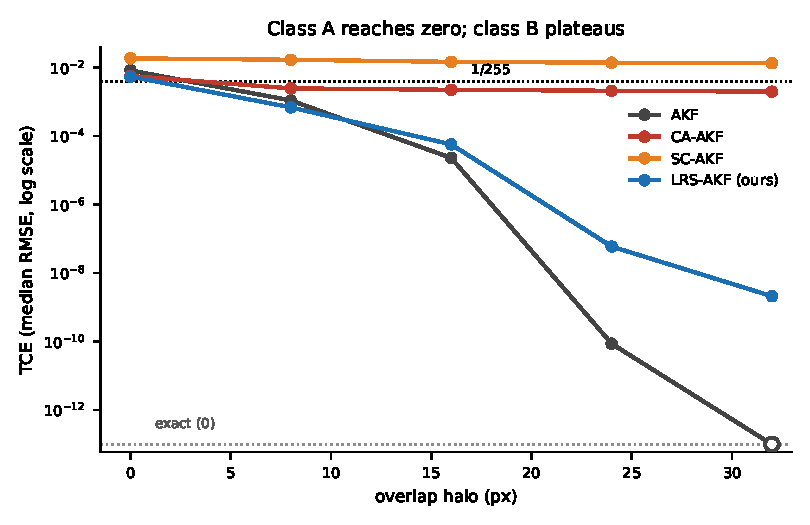
\includegraphics[width=0.82\textwidth]{figures/F1_tce_halo.pdf}
\caption{Two bounded-support operators reach the exact floor as the overlap halo grows, while the two global-quantile configurations plateau. Median tile-consistency RMSE over ten images at $384\times384$, $4\times4$ grid, logarithmic axis; open circles mark exact zero. The plateau is the class-B signature: at halo 32 the global configurations still leave 6.5\\,\% and 20.5\\,\% of pixels differing by more than one 8-bit level, in tile interiors.}
\label{fig:ladder}
\end{figure*}

\section{Results}\label{sec:results}

All measurements use public-domain images from The Metropolitan Museum of Art Open Access programme (CC0, licence evidence recorded per image) at \(384\times384\). Comparisons are paired over the same images; we use two-sided Wilcoxon signed-rank tests and Holm adjustment within two pre-specified families, the \emph{consistency family} (RMSE, \(\mathrm{frac}_{1/255}\), \(\mathrm{frac}_{4/255}\), mean and worst-pixel deviation) and the \emph{quality family} (SR, SSIM, FSR, ECE, SCG, OVT). At \(n=10\) the smallest attainable two-sided \(p\) is \(0.00195\). We therefore report the per-image win rate, the paired effect size \(d_z\) and a paired-bootstrap 95\,\% interval for the mean difference alongside every \(p\)-value, so that a floored \(p\)-value is not mistaken for a small effect.

\subsection{The global-quantile configuration is not tile-consistent}\label{the-global-quantile-configuration-is-not-tile-consistent}

Figure~\ref{fig:ladder} and Table~\ref{tab:ladder} give the halo ladder. The two local operators decay to machine exactness: at halo 32 the tiled LRS-AKF output differs from the whole-image output by at most \(4\times10^{-6}\) on a \([0,1]\) scale, one thousandth of a display level, on every one of the ten images. The two global-statistic operators plateau: doubling the halo from 16 to 32 px reduces their TCE by 9--14\,\%, and at halo 32 6.5\,\% (CA-AKF) and 20.5\,\% (SC-AKF) of pixels still differ by more than one 8-bit level, with worst single-pixel deviations of 21 and 158 display levels.

\begin{table*}[t]
\caption{Median tile-consistency RMSE against overlap halo on ten images at $384\times384$ ($4\times4$ grid), with the fraction of pixels differing by more than one 8-bit level and the worst single-pixel deviation at halo 32. The two bounded-support operators reach the exact floor; the two global-quantile operators do not.}
\label{tab:ladder}
\centering
\footnotesize
\begin{tabular}{@{}lccccccc@{}}
\toprule
method & h=0 & h=8 & h=16 & h=24 & h=32 & frac$>1/255$ & worst $\max D$ \\
\midrule
AKF (fixed radius, local control) & 8.28e-3 & 1.10e-3 & 2.31e-5 & 8.73e-11 & \textbf{0.0} & 0.0000 & 9e-13 \\
CA-AKF (global quantile) & 5.69e-3 & 2.48e-3 & 2.25e-3 & 2.11e-3 & \textbf{1.99e-3} & \textbf{0.0652} & 8.28e-2 \\
SC-AKF (global quantile, tuned) & 1.87e-2 & 1.70e-2 & 1.47e-2 & 1.39e-2 & \textbf{1.34e-2} & \textbf{0.2055} & 6.18e-1 \\
LRS-AKF (ours, final) & 5.49e-3 & 6.91e-4 & 5.74e-5 & 5.98e-8 & \textbf{2.12e-9} & 0.0000 & 4e-6 \\
\bottomrule
\end{tabular}
\end{table*}

The residual lives in tile \emph{interiors}, not on the seams. At \(n=8\) and halo 16, the mean deviation per border band is flat for CA-AKF (1.75e-3 to 2.00e-3 from the grid line outwards) and for SC-AKF (8.1e-3 to 9.7e-3), while the fixed-radius control is confined to the first band. Grid-line visibility is 0.016 (concentration 1.0) and 0.017 (1.1) for the class-B operators against 0.221 (14.2) for the control. One is a genuine seam that a blender could hide; the other is spread through the image and cannot be.

\subsection{Quality: a trade-off, reported with effect sizes}\label{quality-a-trade-off-reported-with-effect-sizes}

Table~\ref{tab:quality} gives the six-metric family. In the primary cohort of ten images, LRS-AKF is significantly better on SSIM and SCG, significantly worse on FSR, and not distinguishable on SR, ECE or OVT after Holm correction. The two surviving gains and the one surviving regression have \(|d_z|>1\) and bootstrap intervals well away from zero (SSIM \(d_z=3.41\), FSR \(d_z=2.64\)). OVT is the informative disagreement: its mean-difference interval excludes zero (\([-0.0057,-0.0001]\)) while the rank test does not reject (\(p=0.137\)), which is what a skewed metric with one large pair looks like. We keep OVT in the indistinguishable group because the pre-specified family test decides significance. The interval describes the mean; the rank test decides the claim, and reporting both keeps the resolution floor visible. Section~\ref{sec:replication} shows that this borderline OVT interval does not survive replication.

\begin{table*}[t]
\caption{Paired quality comparison of CA-AKF (global-quantile reference) against LRS-AKF (final) over ten images: mean $\pm$ sample sd, paired mean difference $\Delta$, paired effect size $d_z$, a 95\\,\% paired-bootstrap interval for $\Delta$ (20,000 resamples, seed 20261104), images won, and two-sided Wilcoxon $p$ with Holm-adjusted value. SR/SSIM/SCG higher is better; FSR/ECE/OVT lower is better.}
\label{tab:quality}
\centering
\footnotesize
\begin{tabular}{@{}lcccrccrr@{}}
\toprule
metric & CA-AKF & LRS-AKF & $\Delta$ & $d_z$ & 95\\,\% CI of $\Delta$ & win/10 & $p$ & $p_{\mathrm{Holm}}$ \\
\midrule
SR & 0.5353 $\pm$ 0.087 & \textbf{0.5656 $\pm$ 0.097} & +0.030 & +0.68 & [+0.0020, +0.0544] & 8 & 0.084 & 0.168 \\
SSIM & 0.6904 $\pm$ 0.079 & \textbf{0.7259 $\pm$ 0.081} & +0.036 & +3.41 & [+0.0295, +0.0416] & 10 & 0.00195 & \textbf{0.012} \\
FSR & \textbf{0.1981 $\pm$ 0.056} & 0.2287 $\pm$ 0.065 & +0.031 (worse) & +2.64 & [+0.0236, +0.0371] & 0 & 0.00195 & \textbf{0.012} \\
ECE & 18.08 $\pm$ 4.18 & \textbf{17.20 $\pm$ 4.10} & $-$0.88 & $-$1.05 & [$-$1.3795, $-$0.4038] & 7 & 0.027 & 0.082 \\
SCG & 0.0756 $\pm$ 0.017 & \textbf{0.0858 $\pm$ 0.018} & +0.010 & +1.01 & [+0.0047, +0.0165] & 8 & 0.0098 & \textbf{0.039} \\
OVT & 0.0069 $\pm$ 0.008 & \textbf{0.0043 $\pm$ 0.004} & $-$0.003 & $-$0.52 & [$-$0.0057, $-$0.0001] & 6 & 0.137 & 0.168 \\
\bottomrule
\end{tabular}
\end{table*}

The FSR regression is expected and is a genuine trade-off. The local reference is a \emph{relative} quantity, so with \(c=1\) the operator is more conservative about growing the support in flat regions and retains more high-frequency texture where the global threshold paints flat. It is controllable by \(c\), which moves FSR back toward the baseline while leaving tile consistency untouched: consistency is a property of the \emph{support} of the parameter chain, not of its threshold value. Figure~\ref{fig:gallery} shows the mechanism directly: in the flattest \(96\times96\) window of a museum image, the bounded-support operator retains more high-frequency texture, which is what a higher FSR measures. We do not claim LRS-AKF is better on every metric, and we do not treat a trade-off as a win.

\begin{figure*}[t]
\centering
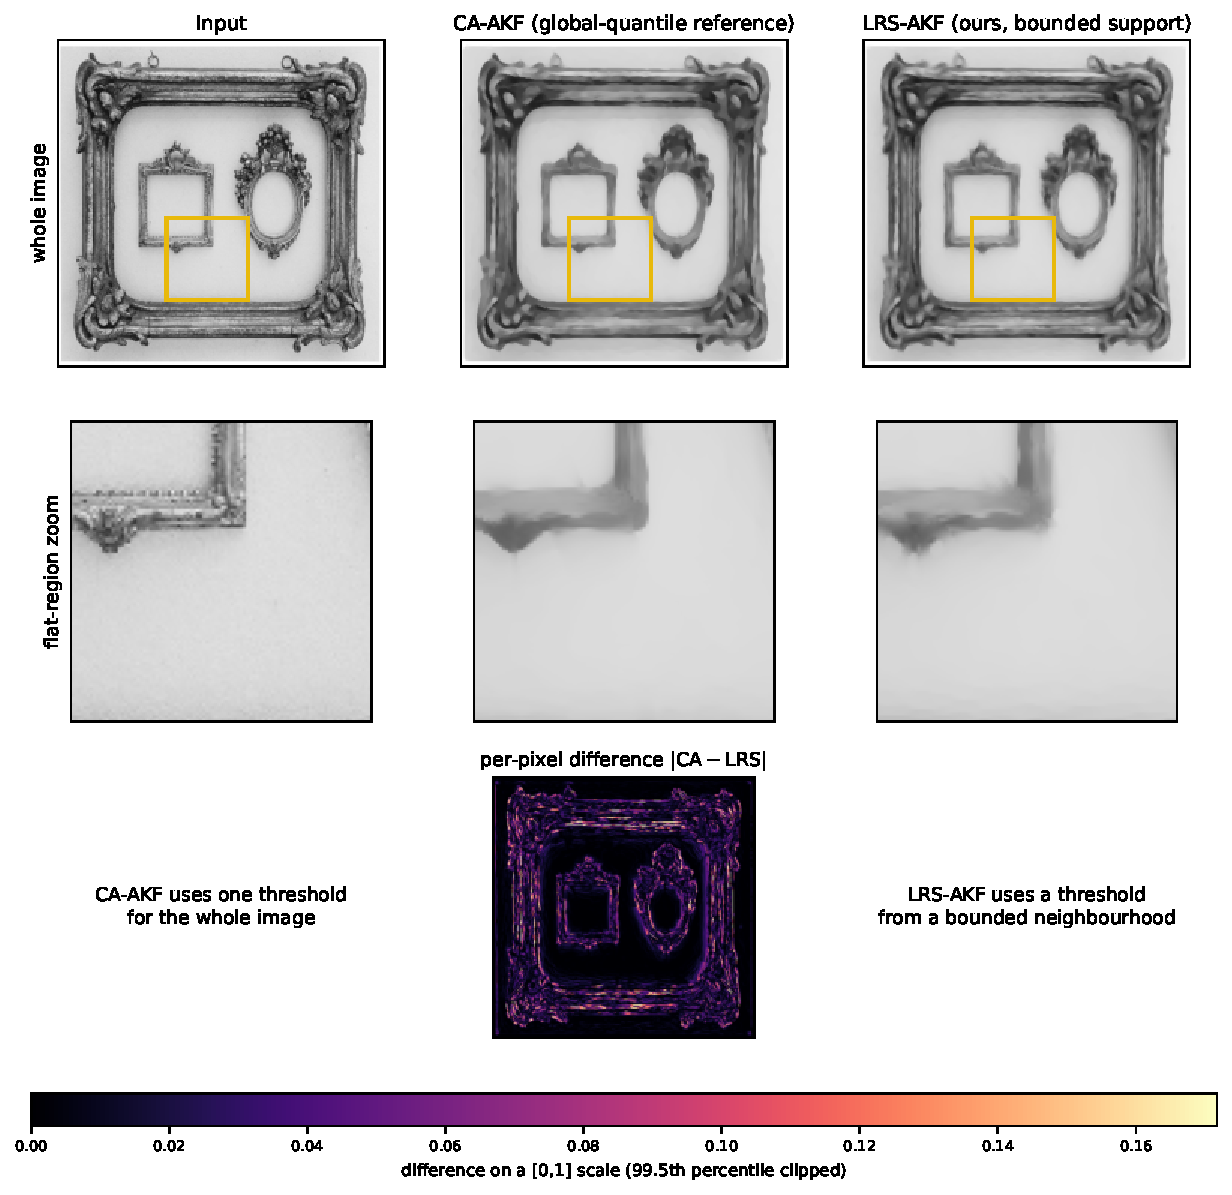
\includegraphics[width=0.73\textwidth]{figures/F10_gallery.pdf}
\caption{The bounded-support operator retains more high-frequency texture in flat regions, the mechanism behind its higher FSR; the marked box is the flattest $96\times96$ window by gradient energy. Top row: input, the global-quantile reference and LRS-AKF. Middle row: the marked window enlarged. Bottom: per-pixel difference between the two outputs. Table~\ref{tab:quality} reports the same trade-off numerically (SSIM $+0.036$, FSR $+0.031$ worse). The two outputs are visually close, which is why six established metrics disagree on which is better.}
\label{fig:gallery}
\end{figure*}

\subsection{The consequence for published numbers}\label{the-consequence-for-published-numbers}

Every method was evaluated under both harnesses on the same images. Whole-image values for CA-AKF and LRS-AKF are in Table~\ref{tab:quality}; those for SC-AKF are SR 0.5147, SSIM 0.6983 and ECE 18.6882. Table~\ref{tab:portability} reports the consequence of the change. SC-AKF loses \(0.031\) SR, \(0.019\) SSIM and \(0.009\) SCG and worsens ECE by \(0.40\) under tile-wise evaluation; its whole-image SSIM edge over CA-AKF is \(+0.0079\), and the same two operators evaluated tile-wise differ by \(-0.0137\). The sign of a headline quality claim reverses under a harness change, on a move no reviewer would call an effect size. AKF and LRS-AKF move by zero to the four decimals reported (largest residual \(1.2\times10^{-4}\)). Across four metrics and ten images, evaluating the same four filters tile-wise instead of whole-image inverts the ranking in 15 of 40 cases (Figure~\ref{fig:rank}).

\begin{table*}[t]
\caption{Change in each quality metric when evaluation moves from whole-image to tile-wise on the same ten images ($\Delta$ = tiled minus whole). SC-AKF's apparent quality is a property of the harness, not of the operator; the two bounded-support operators are unchanged at the reported precision, with a largest residual of $1.2\times10^{-4}$.}
\label{tab:portability}
\centering
\footnotesize
\begin{tabular}{@{}lrrrrrr@{}}
\toprule
method & $\Delta$SR & $\Delta$SSIM & $\Delta$SCG & $\Delta$ECE & $\Delta$OVT & $\Delta$FSR \\
\midrule
AKF & +0.0000 & $-$0.0000 & +0.0000 & +0.0000 & +0.0000 & $-$0.0001 \\
CA-AKF & +0.0004 & +0.0025 & +0.0012 & $-$0.0017 & $-$0.0009 & +0.0000 \\
SC-AKF & \textbf{$-$0.0310} & \textbf{$-$0.0191} & $-$0.0086 & \textbf{+0.4029} & +0.0132 & $-$0.0091 \\
LRS-AKF (ours) & +0.0000 & +0.0000 & $-$0.0000 & +0.0001 & +0.0000 & +0.0000 \\
\bottomrule
\end{tabular}
\end{table*}

\begin{figure*}[t]
\centering
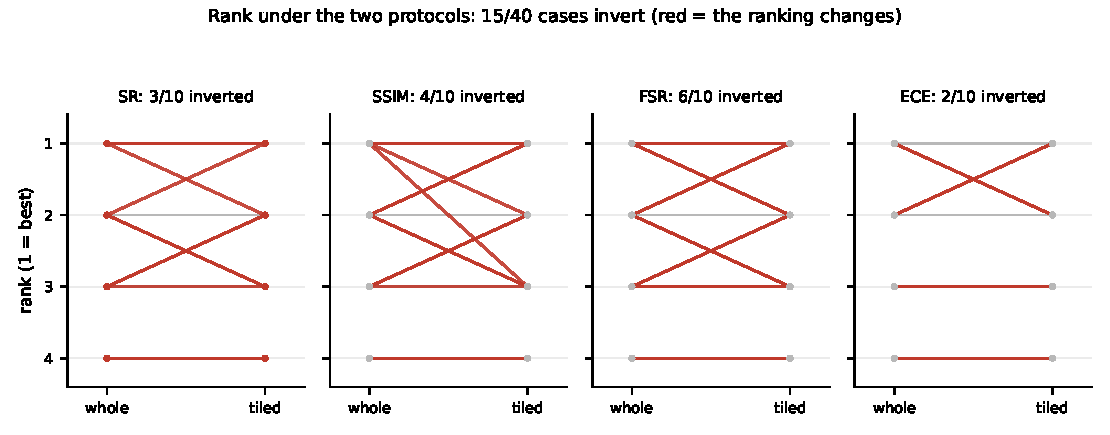
\includegraphics[width=0.82\textwidth]{figures/F5_rank_flip.pdf}
\caption{Method ranking under whole-image versus tile-wise evaluation of the same ten images. One panel per metric, rank 1 = best; each line follows one method's rank between protocols, grey where unchanged and red where it changes. Fifteen of the 40 image-metric cases invert, on metric moves as small as $0.0025$.}
\label{fig:rank}
\end{figure*}

These columns are not a quality ranking. SC-AKF remains a legitimate perceptual configuration whose global quantile was tuned on whole-image statistics. The point is that its reported quality is not portable, while ours is. An exactly tile-consistent operator's published numbers cannot be perturbed by another group's evaluation harness: this is the sense in which the contribution is metrological, and it is the one claim here that the six quality metrics are blind to.

\subsection{Breadth and deployment scale}\label{breadth-and-deployment-scale}

On 144 images (112 museum records, ten bundled scikit-image references, 22 synthetic phantoms) the central claim replicates. At halo 32 the median fraction of pixels differing by more than one level is 6.19\,\% (CA-AKF) and 12.77\,\% (SC-AKF) on the museum records, against 0.00\,\% for LRS-AKF, which is exact on 110/112 museum records and 141/144 overall (three exceptions, one pixel each at 1.2--3.3 levels). No class-B operator is exactly reproducible on more than 6 of the 112 records. The halo ladder is not monotone for them: 10/144 images get worse from halo 16 to 32 for CA-AKF and 27/144 for SC-AKF, against 0/144 for both bounded-support operators, so overlap cannot be tuned towards correctness. The breadth claim is a \emph{single-endpoint} claim with the endpoint pre-specified; the large \(n\) is not bought with additional testing.

At deployment scale the asymmetry becomes practical. On a \(2048\times2048\) mosaic the tiled pass costs 1.36--2.23\(\times\) the time of the whole pass but 4.9--8.9\(\times\) less peak memory, consistent with the bound \(W_{\mathrm{tiled}}\le(1+2h/T)^2W_{\mathrm{whole}}+Nc_0\) for \(N\) tiles of side \(T\) at halo \(h\). A \(4096\times4096\) whole-canvas pass is terminated by the kernel OOM killer on an 8 GB host while the tiled pass completes in 995 MB. On a single artwork at its native \(4000\times3853\) scan, every whole-canvas pass aborts with a 2.07 GiB allocation while every tiled pass completes. At that scale the reference against which the literature measures correctness does not exist, and the pipeline that can run is the one that, for a class-B operator, returns a different image.

\subsection{Third-party code}\label{third-party-code}

Every operator so far is one we wrote, which leaves the suspicion that the taxonomy describes our code. Table~\ref{tab:thirdparty} runs the identical protocol against seven algorithms as shipped in OpenCV 5.0.0 and opencv\_contrib 5.0.0, on the same 144 images, at one documented setting each and with a support bound registered before the ladder was measured~\cite{tomasi1998bilateral,he2010guided,buades2005nlm,perona1991diffusion,gastal2012amf,zhang2014rollingguidance,xu2011l0smooth}. These are denoisers and smoothers, not abstraction filters; the section establishes that the two classes are observable and correctly predicted in published code, not a quality ranking.

\begin{table*}[t]
\caption{Seven published algorithms on 144 images at one documented setting each, with a support bound registered before measurement. Three bounded-support methods are bit-exact inside their predicted halo on every image; two global-solve methods are not exact on 141 of 144 even at halo 48. GV is grid-line visibility at halo 16.}
\label{tab:thirdparty}
\centering
\footnotesize
\begin{tabular}{@{}lcccccc@{}}
\toprule
method & predicted $\to$ measured halo & exact within / never at 48 & frac$>1$ lv, halo 0 $\to$ 48 & worst px & GV & class \\
\midrule
bilateral & 5 $\to$ 4 & 144/144, 0 & 3.32\\,\% $\to$ 0.000\\,\% & 0.0 & n/a & A \\
guided & 32 $\to$ 32 & 144/144, 0 & 18.44\\,\% $\to$ 0.000\\,\% & 0.0 & 6.72 & A \\
non-local means & 30 $\to$ 16 & 144/144, 0 & 12.03\\,\% $\to$ 0.000\\,\% & 0.0 & n/a & A \\
adaptive manifolds & 36 $\to$ none & 8/144, 132 & 12.71\\,\% $\to$ 0.015\\,\% & 3.0 & 3.58 & A, bound missed \\
rolling guidance & none $\to$ 48 & n/a, 26 & 13.75\\,\% $\to$ 0.000\\,\% & 1.0 & 6.25 & B, global solve \\
L0 smoothing & none $\to$ none & n/a, 141 & 99.95\\,\% $\to$ 99.877\\,\% & 208.5 & 1.00 & B, global solve \\
Perona-Malik & 20 $\to$ none & 0/144, 144 & 51.57\\,\% $\to$ 14.758\\,\% & 193.5 & 0.57 & third failure mode \\
\bottomrule
\end{tabular}
\end{table*}

Class A is the norm and the pre-registered bounds hold for the three bounded-support methods; non-local means converges earlier than the naive stencil count predicts, so the bound is sufficient, not tight. Class B is real in third-party code: L0 smoothing solves a global gradient-domain system and is not exactly reproducible at any halo on 141/144 images, with 99.877\,\% of pixels wrong at halo 48 and grid-line visibility 1.00. A third failure mode lies outside the taxonomy. On 40 images probed, six implementations return bit-identical output for identical content; \texttt{anisotropicDiffusion} does not, on 40/40 images, with a median of 262 pixels differing. One iteration is bit-exact, two or more are not, and the divergence persists with \texttt{cv2.setNumThreads(1)}. We report this as a measured property of a released version, not as a diagnosis, and we do not claim to be the first to observe it.

\begin{figure*}[t]
\centering
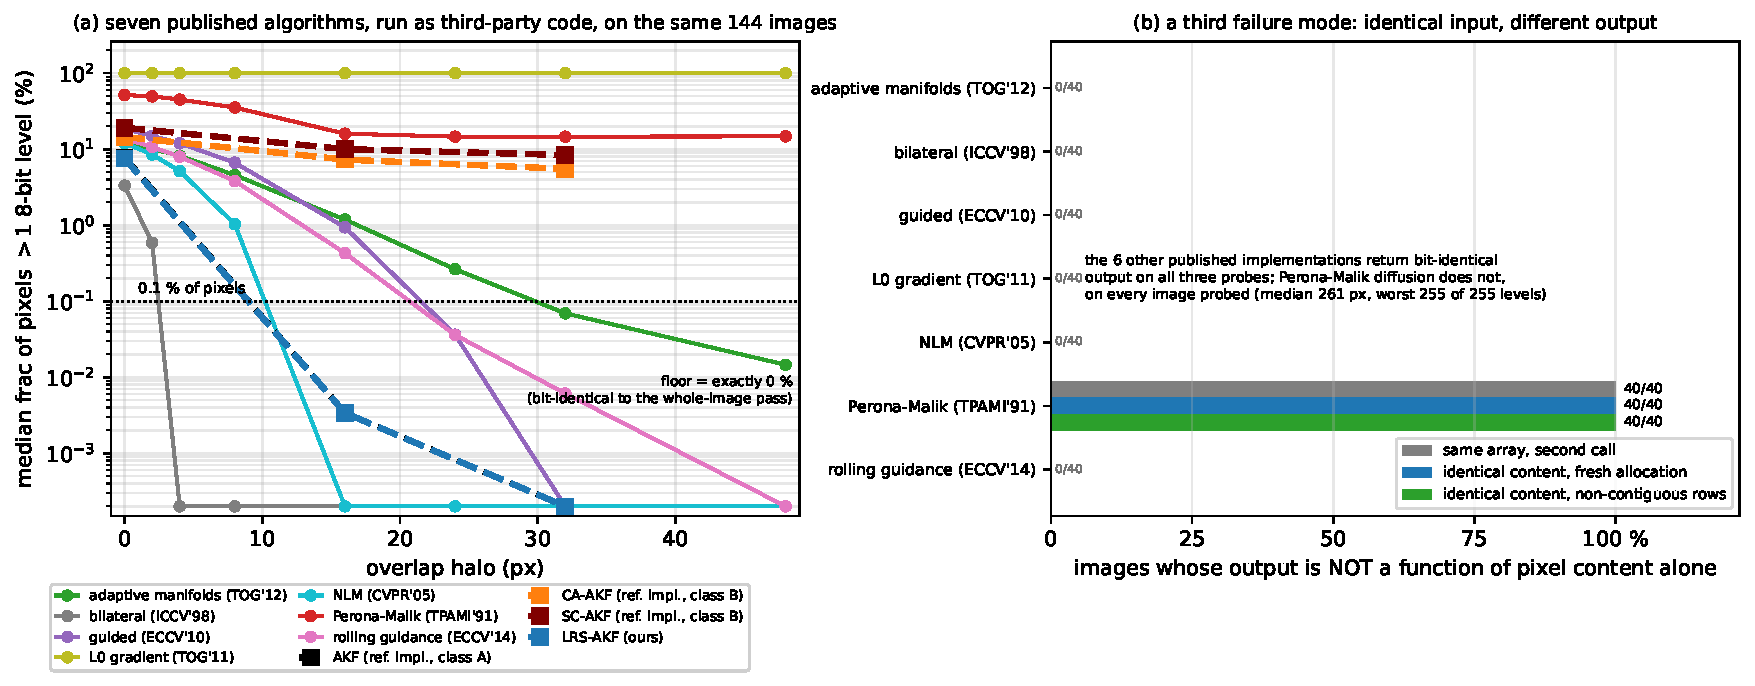
\includegraphics[width=0.82\textwidth]{figures/F9_cv.pdf}
\caption{(a) Median fraction of pixels differing by more than one 8-bit level against overlap halo for seven published algorithms on 144 images; the three bounded-support methods reach zero, the global-solve methods do not. (b) Determinism control: six implementations return bit-identical output for identical content; Perona-Malik diffusion does not, on every image probed.}
\label{fig:thirdparty}
\end{figure*}

\subsection{An audit of distributed implementations}\label{sec:audit}

Section~\ref{sec:results}E establishes that the classes are observable in published code, but none of its seven operators is a Kuwahara variant. We therefore read the expression that forms the parameter in every distributed anisotropic-Kuwahara implementation we could obtain in source form, and recorded the domain over which each expression reduces the image (Table~\ref{tab:audit}). This is a source audit, not a re-run: three of the four are Qt/GLSL or TouchDesigner projects that we could not build on this host, and a build we did not run is not reported as a measurement. One further candidate archive could not be read (its endpoint returned an HTTP 404 body) and is excluded rather than counted.

\begin{table*}[t]
\caption{Parameter chains of four distributed anisotropic-Kuwahara implementations. The reduction domain is the set of pixels whose values enter the expression that sets a pixel's output. Three trees were read as source; the fourth ships only compiled operator files. Exact line ranges are released with the paper.}
\label{tab:audit}
\centering
\footnotesize
\begin{tabular}{@{}p{0.20\textwidth}p{0.15\textwidth}p{0.35\textwidth}p{0.18\textwidth}c@{}}
\toprule
implementation and relation & source read & expression that forms the parameter & reduction domain & class \\
\midrule
\texttt{gpuakf} (2009), independent & \texttt{akf\_v2.glsl}, \texttt{tfm.glsl}, \texttt{glview.cpp} & sector variance $\sigma^2$; weight $1/(1+(255\sigma^2)^{q/2})$; anisotropy from the local structure tensor. \texttt{radius}, \texttt{q}, \texttt{alpha} are UI uniforms & bounded by twice \texttt{radius} & A \\
\texttt{polyakf} (2010), independent & \texttt{akf\_v2n4.glsl}, \texttt{polyakf.cpp} & polynomial weight $1/(1+(255\sigma)^q)$ from sector standard deviations; uniform-only parameters & bounded & A \\
TD-Anisotropic-Kuwahara (2017), independent & \texttt{README.md}, four \texttt{.tox} binaries & declares a port of \texttt{gpuakf}; ships no readable shader text and reports kernel generation as unfinished & inherited by declaration, not verified & A* \\
JLR-CAKF operator base, predecessor project imported by our two references & \texttt{filters.py}, \texttt{repair.py}, \texttt{methods.py} & sector scale is a per-pixel median across $K$ sectors; the structure-repair line mask is thresholded at an image-wide 99th percentile & bounded on the support path, whole-image on the repair branch & A/B \\
\bottomrule
\multicolumn{5}{l}{\footnotesize *Declared inheritance only; the shader text was not available for inspection.}
\end{tabular}
\end{table*}

Three findings follow. First, on the main support-selection path, none of the four uses a whole-image reduction. The published implementations are class-A by construction, and Proposition~1 describes what they already do; our two class-B references are deliberately constructed variants, not recovered examples of a widespread bug. Second, the pattern is not confined to code we wrote: the structure-repair branch of the predecessor pipeline uses an image-wide 99th percentile as a mask threshold, and Section~\ref{sec:results}E finds two OpenCV algorithms with a global solve whose behaviour the class-B prediction describes. Third, the audit is bounded. Four implementations, one release of each, three read rather than executed, do not support a prevalence claim, and we withdraw the one made in earlier drafts. The contribution is a correctness criterion, an instrument that detects a violation in code we did not write, and a measured consequence for reported numbers. None requires the violating pattern to be common.

\subsection{Independent replication on a second numeric stack}\label{sec:replication}

The primary tables were produced on a Linux host (Python 3.12.13). We rebuilt the same operator stack on Windows (Python 3.13.14, numpy 2.5.3, scipy 1.18.1, scikit-image 0.26.0, OpenCV 5.0.0), verified that the operator source files and the image hashes are identical, and re-ran the full battery on 23 images: the ten images of the primary cohort plus 13 new museum records. A same-image check does not reach bit-exactness across the two stacks (median relative drift 0.07 \% for CA-AKF and 12 \% for LRS-AKF, the latter on an RMSE of order \(10^{-4}\)), so this is reported as an independent replication on a second numeric stack, not as an extension of the primary quality table. All 23 images were run in one environment, so the statistics below are internally homogeneous.

\begin{table*}[t]
\caption{Quality family on the independent replication cohort of 23 images (ten shared with the primary cohort, 13 new). Mean $\pm$ sample sd, paired mean difference $\Delta$, paired effect size $d_z$, 95\\,\% paired-bootstrap interval, images won, and two-sided Wilcoxon $p$ with Holm-adjusted value. All six differences keep the sign of the primary table.}
\label{tab:replication}
\centering
\footnotesize
\begin{tabular}{@{}lcccrccrr@{}}
\toprule
metric & CA-AKF & LRS-AKF & $\Delta$ & $d_z$ & 95\\,\% CI of $\Delta$ & win/23 & $p$ & $p_{\mathrm{Holm}}$ \\
\midrule
SR & 0.5522 $\pm$ 0.096 & 0.5867 $\pm$ 0.093 & +0.0345 & +0.80 & [+0.0163, +0.0504] & 20/23 & 0.0024 & 0.0072 \\
SSIM & 0.7109 $\pm$ 0.107 & 0.7417 $\pm$ 0.104 & +0.0308 & +2.28 & [+0.0255, +0.0364] & 23/23 & 2.7e-05 & 0.00016 \\
FSR & 0.1875 $\pm$ 0.058 & 0.2157 $\pm$ 0.067 & +0.0281 (worse) & +1.10 & [+0.0197, +0.0398] & 1/23 & 3.1e-05 & 0.00016 \\
ECE & 19.3344 $\pm$ 6.072 & 18.4710 $\pm$ 5.939 & -0.8634 & -0.68 & [-1.3312, -0.3080] & 18/23 & 0.00085 & 0.0034 \\
SCG & 0.0929 $\pm$ 0.035 & 0.0999 $\pm$ 0.030 & +0.0070 & +0.61 & [+0.0023, +0.0116] & 16/23 & 0.0067 & 0.0134 \\
OVT & 0.0044 $\pm$ 0.005 & 0.0049 $\pm$ 0.004 & +0.0005 & +0.11 & [-0.0015, +0.0024] & 9/23 & 0.4379 & 0.4379 \\
\bottomrule
\end{tabular}
\end{table*}

All six paired differences keep the sign of the primary table, and the smallest two-sided Wilcoxon \(p\) is \(2.7e-05\) rather than the \(0.00195\) floor. Five of the six metrics survive Holm correction. Two conclusions change with the added power, and both are reported rather than smoothed over. SR, ECE and SCG, indistinguishable at \(n=10\), are now significant in the same direction, so the conservative reading of the primary table understates those effects. OVT does the opposite: its \(n=10\) bootstrap interval excluded zero while the rank test did not reject, and in the replication the interval is \([-0.0015, +0.0024]\) with \(p=0.438\). The apparent OVT effect was a small-sample artefact, which is why both statistics are reported for every metric. The consistency claim also replicates: median RMSE at \(n=8\), halo 16 is \(3.70e-03\) for CA-AKF against \(9.83e-05\) for LRS-AKF (paired \(p=2.4e-07\)), and the harness result is stronger than in the primary cohort: SC-AKF's ECE moves by \(+1.22\) on average, while the two bounded-support operators move by at most \(0.0032\) on any metric.

\section{Limitations}\label{sec:limits}

\emph{Threshold.} One 8-bit level as the noticeable unit is a convention, not a perceptual study. The class-A/class-B distinction does not depend on it, since the cases differ in whether the error vanishes as the halo grows, not in how large it is at one threshold. We did not run a perceptual study, so all width claims are statements about a quantisation threshold.

\emph{Image set.} The released benchmark is 286 images: 254 CC0 museum records across four departments, ten bundled public-domain references and 22 deterministic synthetic phantoms. The pool is an acquisition ceiling, not a sampling design: the museum API rate-limited repeated paging, and 254 licence-verified records is what we could retrieve. Served files are normalised to a longest side of 1024 px, so the pool contains no native-resolution image by design; the native experiments use one artwork. Every image is art, photography, costume or a phantom. The design rule is stated for any operator whose parameter is normalised by a global statistic, which includes remote-sensing and histopathology pipelines; we have not run those domains and do not claim their validation.

\emph{Baselines and evidence.} CA-AKF and SC-AKF are reference implementations of the design pattern, not published methods: each builds the same pipeline and differs only in that its threshold is a functional of the whole image. Section~\ref{sec:results}E measures seven published algorithms in third-party code, and Section~\ref{sec:audit} reads four distributed implementations. Both are samples, not a census. Third-party evidence is version-pinned to OpenCV 5.0.0 at one documented setting per method, and the pre-registered support bounds are our reading of each published construction, not the library's claim.

\emph{Statistical resolution.} The quality family is measured on ten images, where the Wilcoxon statistic sits on its resolution floor. We report effect sizes and bootstrap intervals so that a floored \(p\)-value is not mistaken for a small effect. Section~\ref{sec:replication} reports an independent cross-platform replication on 23 images; it is a replication on a second numeric stack, not a pooled sample, because the two stacks do not agree bit-exactly.

\section{Conclusion}\label{sec:conclusion}

We set out a correctness condition for tiled evaluation: a parameter derived from the whole image cannot be used as if it were local. We named the resulting failure mode, separated it from the border artefact that haloes do fix, proved when each case applies and measured both. The condition does not depend on how often the violating pattern is deployed, and Section~\ref{sec:audit} reports that we did not find it on the main support-selection path of the public implementations we could audit.

The operator we introduce replaces a global quantile with a bounded-support local reference. It is exact on 141 of 144 benchmark images, and it pays a real, measured trade-off for that: better on two quality metrics, worse on one, indistinguishable on the rest. It also gains something not otherwise claimable. Its published quality numbers do not move when the evaluation harness changes, whereas a global-statistic variant's SSIM comparison against its sibling flips sign under the same change. Three further results close off attractive-looking routes: the halo ladder is not monotone for a class-B statistic, the sharp reading of the locality proposition is false for real implementations, and the decision statistic is not low-rank. What remains is a design rule, an instrument that makes violations visible at the quantisation floor, an operator that satisfies the rule, and a cost bound saying that tiling buys memory and never time. None of that is a new way to tune a filter.

\section{Data and code availability}\label{data-and-code-availability}

All images are licence-clean and machine-acquired. The 286-image benchmark, its per-object licence manifest, the implementation, the analysis scripts and the unaggregated per-image records behind every table are released with the paper. The anisotropic-Kuwahara operator implementation is included under \texttt{code/reference/} under its original MIT licence, so every sweep can be re-run from this release alone. The third-party benchmark of Section~\ref{sec:results}E drives OpenCV 5.0.0 directly and needs no operator code. The replication cohort of Section~\ref{sec:replication} is released as unaggregated per-image records (\texttt{out/sweep\_replication.jsonl}) with the pinned environment and the cross-platform drift measured on the ten shared images. The four source trees audited in Section~\ref{sec:audit} are archived with content hashes and the exact line ranges quoted in Table~\ref{tab:audit}; three were read as source and none was executed on this host. Code, data and per-image records are available at https://github.com/HwH-1/locality-matters-tile-consistency; the release includes a SHA-256 manifest. \textbf{Funding.} None. \textbf{Competing interests.} None declared. \textbf{Ethics.} Not applicable: the study uses no human subjects, personal data or animal material.

\bibliographystyle{IEEEtran}
\bibliography{refs}
\end{document}
